\section{Itthipaṇḍaka, Animittā, Nimittamattā, Vepurisikā}

There are various other words mentioned in the ordination procedures for {\em Bhikkhunīs} as described in the {\em Bhikkhunikkhandhaka} that are interesting in this context. The last three of these do not exclude an aspirant from ordination:\footnote{Khandhaka 20 Bhikkhunikkhandhaka PTS vol 2 page 271, translated by Ajahn Brahmali.} \\

\begin{tabular}{ l l }
 {\em itthipaṇḍaka} & female {\em paṇḍaka} \\
 {\em animittā } & woman who lacks genitals \\
 {\em nimittamattā } & woman with incomplete genitals \\ 
 {\em vepurisikā } & woman who is manlike \\
\end{tabular} \\

The word {\em animittā} literally means `signless' and appears a number of times in the Canon but mostly with a different meaning, namely as in {\em animitto (ceto)samādhi}, which is translated by Bhikkhu Sujato as `signless immersion', a term used in the context of meditation. In the context of not having genitals, it only appears in the Canon in the {\em Bhikkhunikkhandhaka} and as a form of abuse for women in the {\em Bhikkhu Saṃ­ghā­di­sesa­ 3}; never on its own but always in the same sequence of words of which the above are a few.

The three words  {\em animittā}, {\em nimittamattā} and {\em vepurisikā} do not appear in any of the earlier commentarial texts but appear again in the {\em Tikā Vajirabuddhi / Cūḷavaggavaṇṇanā} without further explanation.

These four terms mentioned in the {\em Bhikkhunikkhandhaka} are rather vague in their descriptions. The Chinese texts are not very clear on this point either but the overall questions asked here seem to be mostly to do with menstruation and diseases. At first glance it seems that the rules regarding ordination are trying to make sure that the girl in question is old enough for ordination and not ill. Rules concerning whether or not a girl has breasts can be explained as a question with regards to age, or it can be explained as a question to find out if she has developed the secondary characteristics needed or is possibly intersex. We will never know the true purpose behind these questions but it is not unlikely that these questions about the development of sexual organs were asked for the sole purpose of establishing age. After all, we also find rules in the {\em Bhikkhunīpātimokkha} that prohibit the ordination of married girls under the age of 12.\footnote{{\em Pācittiya 65 Yā pana bhikkhunī ūnad­vāda­sa­vassaṃ gihigataṃ vuṭṭhāpeyya, pācittiyaṃ.} (``Should any bhikkhuni give Acceptance to a married woman less than twelve years old, it is to be confessed.'', translation by Thanissaro Bhikkhu)} The question about whether a girl is sterile or barren would point to her at least having had one child (how else would they know if she is fertile) but this would seem strange if she wants to enter a celibate Order. It seems likely that the question was intended to establish if she is at least menstruating.

These terms hardly appear in any texts and also not in the earlier commentaries. Bhikkhu \cite{sujato2009} argues that the {\em Bhikkhunikkhandhaka}, as well as other parts of the Vinaya, are a later addition, possibly dating back to the Second Council and the elusiveness of these terms seems to confirm that.

Note that in the Pali, the word used for characteristic is {\em nimitta} and not {\em liṅga} or {\em vyañ­jana} as we would expect. Bhikkhu Sujato points out that the Bhikkhunī Vinaya uses its own language and terminology that is often more in line with the Jain terminology and is poorly integrated with the Bhikkhu Vinaya.\footnote{\cite{sujato2009} page 143–145.} This could explain the discrepancies we see between the Bhikkhu and Bhikkhunī Vinaya in describing certain words pertaining to gender. In any case, the variability and vagueness of these terms with reference to gender do not permit a clear picture. 

The following table gives an overview of the terms:

\bigskip
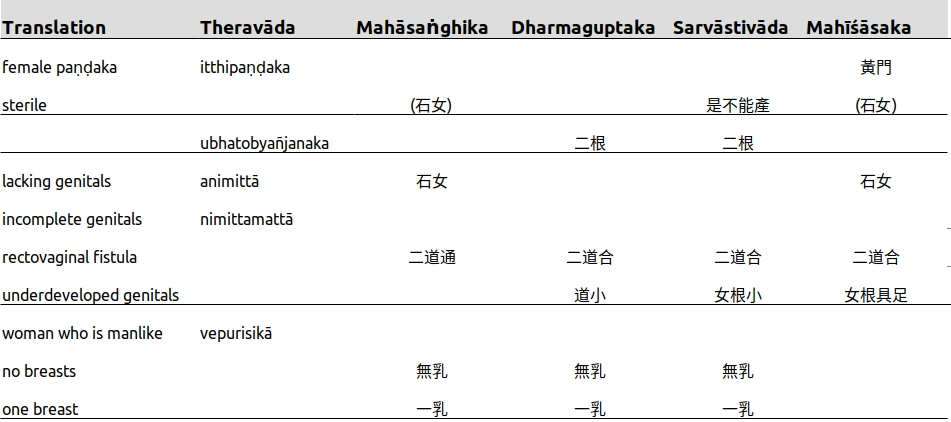
\includegraphics[width=\linewidth]{female.jpg}
\label{female}

It is certain though that the terms {\em paṇḍaka} and {\em ubhatob­yañ­janaka} pertained exclusively to male candidates as we have also seen in the Jain Order while the Bhikkhunī seem to have had their own vocabulary.

There are some rare cases of people who were raised from birth as girls that later became assigned as {\em hijra} after they failed to develop secondary female sexual characteristics (breast development and menstruation) at puberty.\footnote{\cite{nanda} page 15.} Although there is very little evidence to go on, I believe that these cases could possibly be representing the {\em itthipaṇḍaka}. The {\em itthipaṇḍaka} only appears in the Pali scriptures while the Chinese talk about a `barren/sterile woman', which could be the same or not. Only the Mahīśāsaka Vinaya talks about a 黃門 ({\em paṇḍaka}). 

At least in the Bhikkhunī ordination in the Theravāda lineage, the {\em animittā, nimittamattā and vepurisikā} are allowed to ordain. This is possibly also true in several of the Chinese Vinayas.
